\documentclass[twocolumn]{aastex62}

\newcommand{\vdag}{(v)^\dagger}
\newcommand\aastex{AAS\TeX}
\newcommand\latex{La\TeX}
\usepackage{amsmath}
\usepackage{physics}
\usepackage{hyperref}
\usepackage{natbib}
\usepackage[T1]{fontenc}
\usepackage[english]{babel}
\usepackage[utf8]{inputenc}

\begin{document}

\title{\Large Foreløpig ingen tittel.}

\author{Håkon Tansem}

\author{Nils-Ole Stutzer}

\author{Bernhard Nornes Lotsberg}

\begin{abstract}

\end{abstract}

\section{Introduction} \label{sec:intro}
An ever occuring problem in many fields of science is a binary system of
interacting elements taking two possible values. Binary problems can be found in
everything from political science, where one could model outcomes of a vote in a
two party system, to modeling phase transitions in solid states physics. In this
paper we will focus on the latter, where we will model a time evolving
two-dimensional Ising model of interacting spins by means of a Markov Chain
Monte Carlo (MCMC) algorithm in addition to a Metropolis algorithm as described
by Ch. 3. and 4. by \cite{newman:2019}. We will explore how
different grid sizes and temperatures make the lattice behave, and how the systems energy and magnetisation
developes in time, the final aim being to estimate the critical temperature of
the phase transition when the lattice looses its magnetisation, as presented in
Ch. 5. and 6. in \cite{plischke:2006}. This is then
compared to the analytical value found by \cite{onsager:1944}. 

This paper will present needed theory and implementation of the theory in the Method
section \ref{sec:method}, the results will be presented in the Results section
\ref{sec:results} and be discussed in the Discussion section
\ref{sec:discussion}.

\section{Method} \label{sec:method}
\subsection{The Ising Model and Important Quantities from Statistical Menchanics} \label{subsec:ising_model}
The physical system considered by this paper will be a two-dimensional Ising
model, consisting of a grid of $N\times N$ magnetic spins. Each spin can have
the value $s = +1$ or $s = -1$, and they interact only with their nearest neighbours.
The energy of the lattice is defined by the interaction of each neighbouring
spin pair as
\begin{align}
	E = -J\sum_l\sum_{\langle kl\rangle} s_k s_l,
	\label{eq:energy}
\end{align}
where $\langle kl\rangle$ denotes the sum over the nearest neighbours and $J$ has units energy. When counting the
energies we choose to use periodic boundaries, meaning that the nearest
neighbour of a spin $s_{i,N-1}$ at the edge of the lattice is the spin $s_{i,0}$
at the opposite edge of the lattice. This is done so as to simulate a lattice
that extends infinitly in space. 
The magnetisation is defined similarly as 
\begin{align}
	M = \sum_i s_i,	
	\label{eq:magnetisation}
\end{align} 
simply being the sum of the systems spins. The probability density function (PDF) of the system having
a cetain energy state is given by the Boltzmann distribution 
\begin{align}
	P(E_i) = \frac{1}{Z}e^{-\beta E_i},
\end{align}
where $\beta = \frac{1}{k_B T}$ for the Boltzmann constant $k_B$ and the
temperature $T$. The partition function of the system describing all statistical
properties of the system in equilibrium is given as 
\begin{align}
	Z = \sum_{i} e^{-\beta E_i},
\end{align}
over all possible microstates ($2^{N^2}$ in total for a $2\times 2$ grid) of the system. The mean energy and absolute magnetisation
of the system is then given as 
\begin{align}
	\langle E \rangle &= \sum_{i} E_i P(E_i) = \sum_{i} \frac{E_i}{Z}e^{-\beta E_i} = \pdv{\ln Z}{\beta}\\
	\langle |M| \rangle &= \sum_{i} |M_i| P(E_i) = \sum_{i} \frac{|M_i|}{Z}e^{-\beta E_i} 
\end{align}
and represent the most likely state of the system.
Another important quantity from
thermodynamics is the heat capacity measuring the change heat for a given
temperature change. The heat capacity at constant volume is given as 
\begin{align}
	C_V &= \dv{\langle E \rangle}{T} = \frac{1}{k_B T^2}\left(\frac{1}{Z}\sum_{i} E_i^2 e^{-\beta E_i} - \langle E\rangle^2\right) \\
	& = \frac{1}{k_BT^2}\left(\langle E^2\rangle - \langle E\rangle^2\right) = \frac{\sigma^2_E}{k_B T^2},
\end{align}
thus being analogous to the variance in energy states.
Finally, the magnetic susceptibility measuring how the systems magnetisation
responds to a temperature change, is defined as 
\begin{align}
	\chi &= \beta\left(\sum_{i}\frac{M_i^2}{Z}e^{-\beta E_i} - \langle |M_i|\rangle^2 \right)\\
	& = \frac{1}{k_BT}\left(\langle M^2\rangle - \langle |M|\rangle^2\right) = \frac{\sigma^2_{|M|}}{k_BT}.
\end{align} 
These thermodynamical quantities will later be usefull when estimating the
critical temperature of the phase transition when the system looses its net
magnetisation.
When later implementing these thermodynamical quantities numerically we will
use natural units where $k_B = 1$ and the energy is in units $J$, the
temperature will be unitless $k_BT / J$. Also the magnetisation is in
this case a unitless quantity, and due to the energy and temperature scaling the
heat capacity and susceptibility have units $k_B$ and $J^2$ respectively.

\subsection{Analytical Solutions to the $2\times2$ Lattice}\label{subsec:two_by_two_lattice}
Before discribing the algorithm modeling the time development of the lattice, we
show the analytical solutions to the mean energy and absolute magnetisation as
well as the heat capacity and the susceptibility as shown in \ref{subsec:ising_model}, so as to later enable a
comperison of the numerical results to known analytically quantities. When
counting the energy and magnetisation of the $2\times2$ lattice as discribed in
the previous subsection we get the possible states of the system shown in Table
\ref{tab:possible_energy}. This lattice has in all $2^{N^2} = 2^4 = 16$ possible microstates. 

\begin{deluxetable}{cccc}
	%\tablewidth{0pt}
	\tablecaption{Table showing the possible energies $E_i$ and magnetisations $M_i$ of the $2\times2$ lattice and their corresponding number of spins up $N_\uparrow$ and their degenrecies $d_i$. \label{tab:possible_energy}}
	%\tablecomments{}
	\tablecolumns{4}
	\tablehead{$N_\uparrow$ & $d_i$ & $E_i$ $[J]$ & $M_i$}
	\startdata
	$4$  & $1$ & $-8$& $4$   \\
	$3$ & $4$  & $0 $& $2$\\
	$2$ & $4$  & $0 $& $0$\\
	$2$ & $2$  & $8 $& $0$\\
	$1$ & $4$ & $0 $& $-2$\\
	$1$ & $1$ & $-8$ &$-4$ 
	\enddata
\end{deluxetable}
Using the possible energy states in Table \ref{tab:possible_energy} we can write
the partition function of the system as 
\begin{align}
	Z = \sum_{i = 1}^{2^{N^2}} e^{\beta E_i} = 4\cosh(8J\beta) + 12.
\end{align}
Using this we get the expectation value for the energy to be  
\begin{align}\label{eq:analyticalE}
	\langle E\rangle  = \frac{1}{Z}\sum_{i = 1}^{2^{N^2}} E_i e^{-E_i\beta} = -\frac{8J\sinh(8J\beta)}{\cosh(8J\beta) + 3}.
\end{align}
Similarly we find that the expectation value of the absolute magnetisation is
given by 
\begin{align}\label{eq:analyticalM}
	\langle |M| \rangle = \frac{1}{Z}\sum_{i = 1}^{2^{N^2}} |M_i|e^{-E_i\beta} = \frac{2e^{8J\beta} + 4}{\cosh(8J\beta) + 3}.
\end{align}
Next this leads to the heat capacity being 
\begin{align}
	C_V = \dv{\langle E \rangle}{T} = -\frac{1}{k_BT^2}\dv{\langle E\rangle}{\beta} = \frac{192(\cosh(8J\beta) + 1)}{k_B T^2(\cosh(8J\beta) + 3)^2},
\end{align}
and the susceptibility (when using the absolute magnetisation) is 
\begin{align}
	\chi_{|M|} &= \frac{1}{k_BT}\left(\langle M^2 \rangle - \langle |M|\rangle^2 \right) \\
	&= \frac{1}{k_BT}\left(\frac{8e^{8J\beta} + 8}{\cosh(8J\beta) + 3} -\frac{(2e^{8J\beta} + 4)}{(\cosh(8J\beta) + 3)^2} \right).
\end{align}

These analytical quantities can be compares to the numerical results.

\subsection{The MCMC and Metropolis Algorithms}
Now that we have looked at how the lattice of $N\times N$ interacting spins is set up, we
can begin describing the algorithm used to simulate the evolution of the lattice
in time. The algorithm used to simulate the time evolution of the lattice is a
Markov Chain Monte Carlo (MCMC) algorithm. We will, however, only outline the algorithm
used here, which is derived in detail in Ch. 3. and 4. of \cite{newman:2019}.
The main idea behind a Markov Chain is that we want to let the system, in our
case being the lattice of spins, transition from one state $w_i$ to the next state $w_j$
in time. This can be written as 
\begin{align}
	w_j = W(i\to j)w_i,
\end{align}
where $W(i\to j)$ is the transition matrix quantifying the probability
transitioning to $w_j$. If we iterate over many such changes-of-states
the system will converge to the state corresponding to the eigenvector of the
transition probability matrix $W(i\to j)$ having the largest eigenvalue. Since
$W(i\to j)$ is a stochastic matrix, the largest eigenvalue is one. Applying the
matrix to an initial state $w_i$ many times the system thus converges towards equilibrium, effectively loosing the time dependence since the change from each
iteration to the next becomes negligable. This means that effectively
\begin{align}
	w(t_i) - w(t_i + \epsilon) = 0,
\end{align}
for a small change $\epsilon$, near the equilibrium position. This can be
rewritten as 
\begin{align}
	\sum_i W(i \to j)w_i - W(j \to i)w_j = 0,
	\label{eq:sum_of_states}
\end{align}
simply multiplying out the matrix product of the forward and backward
transitions. There are multiple ways (\ref{eq:sum_of_states}) can be fulfilled,
but we impose detailed balance \citep[Ch. 3. and 4.]{newman:2019} so that each element of the sum
fulfills the equation, making
\begin{align}
	W(j \to i)w_j - W(i \to j)w_i = 0.
\end{align}
Now, because we do not know the transition probabilities $W$ because they are
unknown or too complicated to model, we can use the above relation to model the transition
probability using the Metropolis algorithm \citep[Ch. 3. and 4.]{newman:2019}. From the detailed
balance we get that 
\begin{align}
	\frac{w_j}{w_i} = \frac{W(j \to i)}{W(i \to j)} \equiv r.
	\label{eq:trans_prob}
\end{align}
Since the $w$'s are probabilities, the l.h.s. quantifies whether the next state
is more probable than the previous state. Thus if the ratio
$\frac{w_j}{w_i}\geq 1$ we let the system transition to the next state as the
forward transition probability $W(j \to i)$ is larger than the backwards
transition probability $W(i \to j)$. However if the l.h.s. of
(\ref{eq:trans_prob}) is less than one there is a finite probability that the
system may transition forwards or backwards. This must be included in the acceptance rule so as
to not include a bias freezing the system at the state of highest probability,
as we want the system to transition to as many, if not all possible states.

In our case we can rewrite (\ref{eq:trans_prob}) as 

\begin{align}
	r \leq \frac{P(E_2)}{P(E_1)} = \frac{\frac{1}{Z}e^{-\beta E_2}}{\frac{1}{Z}e^{-\beta E_1}} = e^{-\beta\Delta E}, 
\end{align}
where $r\in[0, 1]$ is a number drawn from a uniform distribution, effectively
modeling all transition posibilities and at the same time eliminate the unknown
partition function $Z$. 

When implementing the Markov Chain in practice we first must initialize the
system by computing the $N\times N$ lattice energy and magnetisation.
This is simply done by using (\ref{eq:energy}) and (\ref{eq:magnetisation}) as
described previously.

We simulate the time evolution by looping through a number of $m$ Monte Carlo
cycles. Then at each Monte Carlo cycle we sweep through the lattice $N\times N$
times to roughly cover the whole grid, by picking a random grid point $i, j$
drawn from a uniform distribution $i,j\in[0, N-1]$ using a Mersenne-Twister
pseudo-random number generator, at each sweep. At each sweep we
suggest a spin flip and compute the energy of the lattice after the flip. Since each spin only has four different nearest neighbours
contributiong
to
the energy we find that the change in energy for any suggested flip is among
five possible values $\Delta E \in {-8J, -4J, 0, 4J, 8J}$. Both the change in
energy $\Delta E$ and the change in magnetisation $\Delta M$ from a spin flip have analytical
expression;
\begin{align}
	\Delta E &= E_2 - E_1 = -J\sum_{\langle kl\rangle}s_k^2s_l^2 + J\sum_{\langle kl\rangle}s_k^1s_l^1 \\
	&= -J\sum_{\langle kl\rangle}s_k^2(s_l^2-s_l^1) = 2s_l\sum_{\langle k\rangle} s_k,
\end{align}
since the surrounding spins $s_k = s_k^1 = s_k^2$ are unchanged and the fliped
spin $s_l^2 = -s_l^1$. The magnetisation change is 
\begin{align}
	\Delta M = 2s_l^2,
\end{align}
since the difference in magnetisation at a spin flip is 2. This way of
suggesting a new state is more efficient than to compute the energy diffence
using a whole new lattice configuration, as it requires a lot less FLOPs.

The differnece in energy is than used to deterain whether the suggested spin
flip is accepted or not through the described Metropolis algorithm.

For each accepted spin flip the energy and magnetisation sample means and variances are
updated. After many cycles the system will than converge to the most like state
$\langle E\rangle$, and oscillate around it. 


\subsection{The Analysis}\label{subsec:analysis}
Now that we have an algorithm computing the discribed thermodynamic quantites,
we can compare the output to the known analytical values for a $2\times 2$ grid
for say a temperature $k_BT/J = 1.0$.

The next step would be to choose a larger lattice, for instance $N = 20$, both
with an ordered and disordered initial spin configuration. Then we let the
system run through a large number of Monte Carlo cycles, representing a long
time, and computing the sample mean of energy and absolute magnetisation as
\begin{align}
	\langle E\rangle &= \frac{1}{m}\sum_{i = 1}^m E_i\\
	\langle |M|\rangle &= \frac{1}{m}\sum_{i = 1}^m |M_i|,
\end{align} 
at each Monte Carlo cycle $m$. This cumulative mean we can use to find how much
time, i.e. how many Monte Carlo cycles, the system needs to reach a state close
to the most likely state where $\langle E \rangle$ and $\langle |M|\rangle$
start flattening out. This is deterained by a by-eye estimate. This is used as a
starting time for the later sampling of energies and magnetisation for
the thermodynamical quantites $C_V$ and $\chi$ when looking at the phase
transitions. 
Also we plot the number of accepted flips as a function of the Monte Carlo
cycles to see how much the system changes states at any given time.

To further see if the lattice behaves as expected we can approximate the
Boltzmann distribution $P(E)$ for a given temperature $k_BT/J$ by making a
histogram of the energy states of the system. We would expect that for a low
temperatue like $k_BT / J = 1.0$ that $P(E)$ approaches a $\delta$-function at
small energies as
$\beta$ becomes large, and the exponential function $P(E)$ quickly dies out when
energies become larger. The lattice effectively freezes at the lowest possible
energy state. Therewhile for higher temperatures like $k_BT/J$ the PDF
will look more like a Gaussian distribution as the system has meany more
possible (symmetric) energy states around the equilibrium that it can oscillate
around. 

The distributions are than compared to the sample variance given by the central
limit theorem \citep[p. 357]{jensen:2015} defined as 
\begin{align}
	\sigma^2 = \frac{\sigma^2_E}{m},
\end{align}
for the number of experiments (Monte Carlo cycles) $m$ and the energy variance
$\sigma_E^2 = \langle E^2\rangle - \langle E \rangle^2$. This will be an error
estimate of the statistical experiment as it measures the deviation between the
true mean and the sample mean. Also the spread in the histogram is compared to
the standard diviation $\sigma_E$.

Next, we want to study the phase transition where the lattice looses its net
magnetisation. In the theory presented in Ch. 5. and 6. \cite{plischke:2006} we see that many
physical properties of the system near the
critical temperature can be described by a power law. Near the critical temperature
$T_C$ for when the lattice undergoes the phase transition, the mean magnetisation is
given by 
\begin{align}
	\langle M(T) \rangle \sim (T-T_C)^\beta,
\end{align}
where $\beta = 1/8$ is the so-called critical exponent. The heat capacity and
the susceptibility follow analogous relations as
\begin{align}
	C_V(T) &\sim |T_C - T|^{-\alpha} \\
	\chi(T) &\sim |T_C - T|^{-\gamma},
\end{align}
where $\alpha = 0$ and $\gamma = 7.4$. When the lattice is heated to $T \gg T_C$
the correlation length $\xi$ of the lattice becomes of the order of the lattice size.
The correlation length is a measure of how far two correlated spins are
separated. As the temperatue $T$ appreaches the critical temperature $T_C$, the
correlation length increases as more and more of the lattice spins are correlated, exerting a divergent behaviour close to $T_C$ as 
\begin{align}
	\xi(T) = |T_C - T|^{-\nu},
\end{align}
where we let $\nu = 1$. Since we study a second order phase transition the
correlation length will eventually span the whole system, in our case being
limited to a finite grid this corresponds to the
lattice size $N$. Therefore since
$\xi\propto N$ we get that 
\begin{align}
	T_C(N) - T_C(N\to\infty) = aN^{-1/\nu},
	\label{eq:temp_crit}
\end{align}
where $a$ and $\nu$ are constants. Then the mean magnetisation becomes 
\begin{align}
	\langle M(T)\rangle \sim (T - T_C)^\beta \to N^{-\beta/\nu},
\end{align}
the heat capacity becomes 
\begin{align}
	C_V(T) \sim |T_C - T|^{-\alpha}\to N^{\alpha / \nu}
\end{align}
and the susceptibility is 
\begin{align}
	\chi(T)\sim |T_C - T|^{-\gamma} \to N^{\gamma/\nu},
\end{align}
where we have set $T_C(N) = T$ and $T_C(N\to\infty) = T_C$.
Thus if we plot the mean energy and magnetisation as well as the heat capacity
and susceptibility as a function of temperatres we can estimate the critical
temperature for an infinite grid $N\to \infty$. For this we use $N = 40, 60, 80$
and $100$, and a temperature range of $T\in[2.0, 2.5]$ with 50 temperature steps. We expect that the mean energy
and absolute magnetisation suddenly bend at $T = T_C(N)$, and that the heat
capacity and susceptibility peak at $T = T_C(N)$. When $N\to\infty$ this peak
will diverge. Using (\ref{eq:temp_crit}) for two grid sizes $N_1$ and $N_2$ we
can estimate the constant $a$ to be 
\begin{align}
	a = \frac{T_C(N_1) - T_C(N_2)}{N_1^{-1/\nu} - N_2^{-1/\nu}},
\end{align}
since we know that $T_C(N\to\infty)$ is the same for all grids. Knowing $a$ we
can use (\ref{eq:temp_crit}) to compute an estimate for $T_C(N\to\infty)$. This
estimate can be compared to the analytical value found by \cite{onsager:1944};
$k_BT/J = \frac{2}{\ln(1+\sqrt{2})}\approx 2.269$, for $\nu = 1$.
As looping over several temperatures using a desently large number of Monte
Carlo cycles is very time consuming, we parallelized the temperature loops using
MPI and used compiler flags. To check the speed-up we timed code using diffent
degrees of parallisation and compiler flags.


\section{Results} \label{sec:results}
To determine how many Monte Carlo cycles that were required for the solutions to
stabilize using a $2\times 2$ lattice, the model was compared to the analytical values for the energy and
the absolute magnetization given by (\ref{eq:analyticalE}) and
(\ref{eq:analyticalM}) respectively for a $2\cross 2$ lattice. This shows that the error
became sufficiently small after approximately $10^4$ Monte Carlo cycles.\\
\begin{deluxetable}{lcccc}
	%\tablewidth{0pt}
	\tablecaption{Table showing the mean value for the energy and the absolute magnetization for a $2\cross 2$ lattice. The absolute error computed by comparing the calculated values with the analytical values given by (\ref{eq:analyticalE}) and (\ref{eq:analyticalM}) is also tabulated to illustrate the discrepancy.  \label{tab:error}}
	%\tablecomments{}
	\tablecolumns{5}
	\tablehead{MC cycles  &  $\langle E\rangle$ $[J]$ & $\langle M \rangle$  & $E_{error}$ & $M_{error}$}
	\startdata
	$10$   & $-4.8$    & $2.8$    & $3.183$  & $1.194$  \\
	$10^2$ & $-8.0$    & $4.0$    & $0.016$  & $0.005$  \\
	$10^3$ & $-7.968$  & $3.990$  & $0.015$  & $0.004$  \\
	$10^4$ & $-7.988$  & $3.996$  & $0.004$  & $0.001$  \\
	$10^5$ & $-7.982$  & $3.994$  & $0.0019$ & $0.0006$ \\
	$10^6$ & $-7.9833$ & $3.9944$ & $0.0005$ & $0.0002$
	\enddata
\end{deluxetable}

\begin{deluxetable}{lcccc}
	%\tablewidth{0pt}
	\tablecaption{ Table showing the mean energy and mean absolute magnetization as well as the heat capacity and susceptibility for different temperatures. The values where computed with a number of Monte Carlo cycles of $10^6$. \label{tab:2by2_lattice}}
	%\tablecomments{}
	\tablecolumns{5}
	\tablehead{$k_BT / J$  &  $\langle E\rangle$ $[J]$ & $\langle M \rangle$  & $C_V$ $[k_B]$  & $\chi_{|M|}$ $[J^{-1}]$}
	\startdata
	$1$   & $-7.9841$    & $ 3.9947$    & $0.1263$  & $0.0158$  \\
	$1.28$ & $-7.9086$    & $3.9697$    & $0.4415$  & $0.0698$  \\
	$1.56$ & $-7.7279$  & $3.9096$  & $0.8654$  & $0.1683$  \\
	$1.84$ & $-7.4251$  & $3.8092$  & $1.2673$  & $0.2907$  \\
	$2.12$ & $-7.0192$  & $3.6734$  & $1.5442$ & $0.4131$ \\
	Rel. Error at $\frac{k_BT}{J} = 1.0$ & $4.967 \cdot 10^{-6}$  & $2.780\cdot 10^{-5}$  & $0.003$ & $0.0391$ 
	\enddata
\end{deluxetable}
Using the higherst precision found in Table \ref{tab:error} obtaines with $10^6$
Monte Carlo cycles, we computed the mean energy and absolute value of the
magnetisation as well as the heat capacity and susceptibility for different
temperatures $k_BT/J\in[1.0, 2.12]$. The relative errors to the analytical
solutions described in Section \ref{subsec:two_by_two_lattice} of the computed
quanteties were computed for
the $k_BT/J = 1.0$ case. This is tabulated in Table \ref{tab:2by2_lattice}.

To verify this the model was then used to calculate the energy $E$, absolute
magnetisation $\vert M \vert$ and heat capacity $C_v$ all as functions of the
temperatue $T$ for lattice with size $N=20$. The values were divided by the
lattice area $N^2$ in order to illustrate these quantities per particle. The
number of accepted flips was also counted for these calculations. These results
are shown in figures \ref{fig:E_MC7}, \ref{fig:M_MC7} and \ref{fig:flip_MC7}
respectively. Here we calculated for two separate temperatures $K_B T/ J = 1.0$
and $K_B T/J=2.4$ with two initial spin configurations. One ordered
configuration where all initial spins point in the same direction and a
disordered configuration where all initial spins are randomly chosen.
\begin{figure*}
	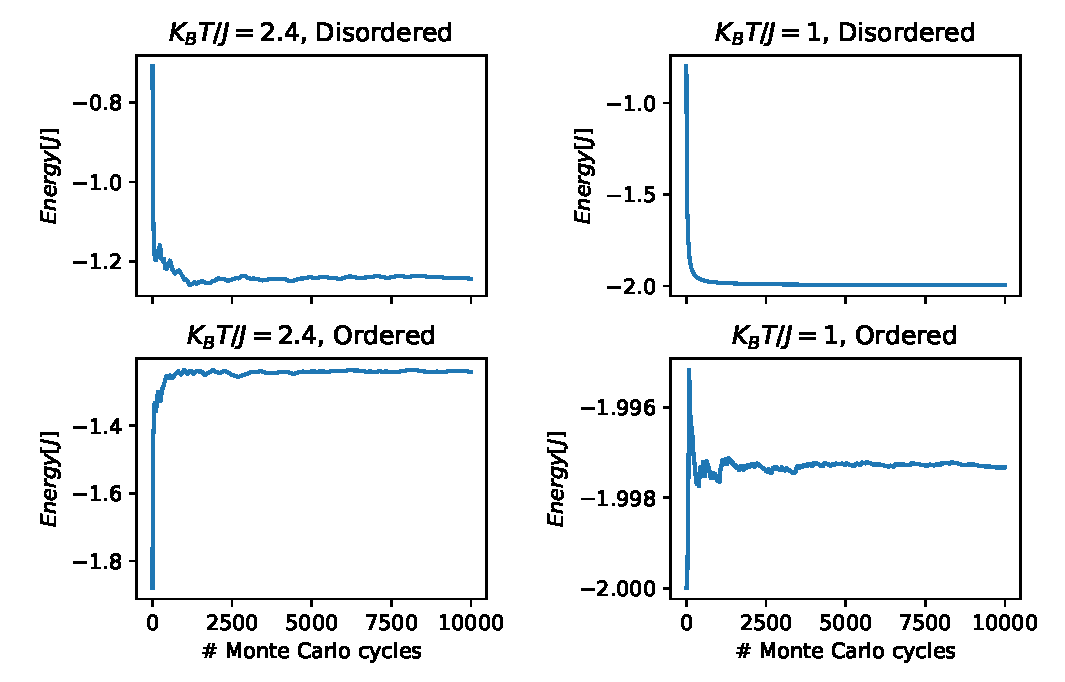
\includegraphics{{Figures/E_MC1e7}.pdf}
	\caption{Figure showing the energy $E$ as a function of Monte Carlo cycles for a lattice with dimensions $N=20$. The simulations were done with two different temperatures $K_B T /J=1$ and $K_B T/J=2.4$ for and ordered lattice where all initial spins point in the same direction and an unordered lattice where all initial spins are chosen randomly.}
	\label{fig:E_MC7}
\end{figure*}

\begin{figure*}
	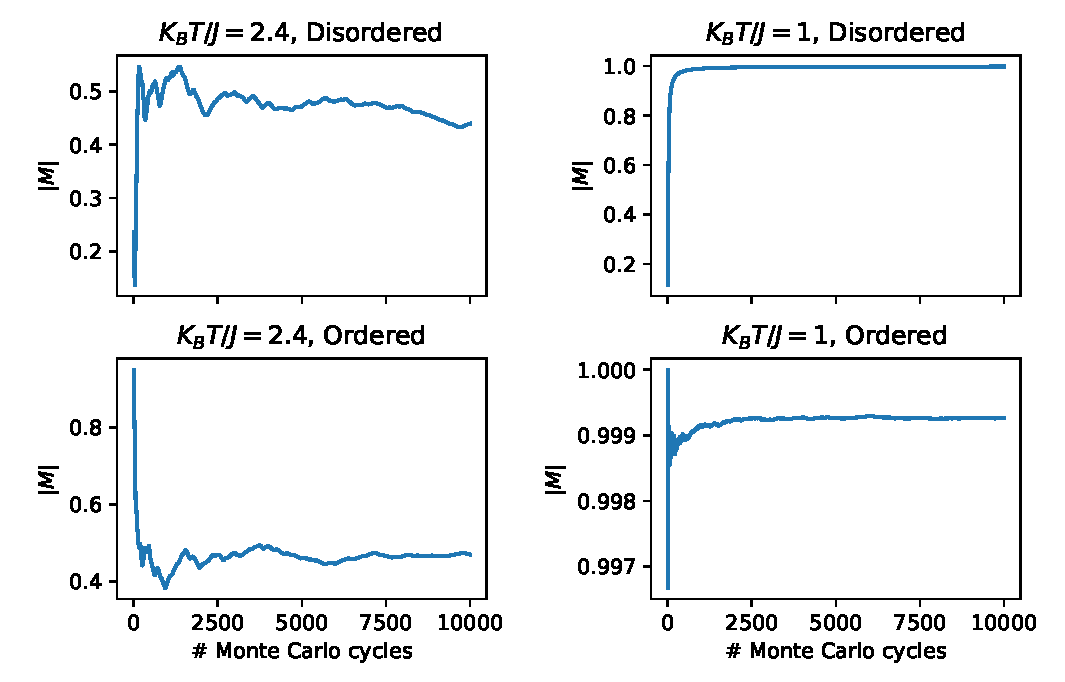
\includegraphics{{Figures/M_MC1e7}.pdf}
	\caption{Figure showing the absolute value of the magnetization $\vert M\vert$ as a function of Monte Carlo cycles for a lattice with dimensions $N=20$. The simulations were done with two different temperatures $K_B T /J=1$ and $K_B T/J=2.4$ for and ordered lattice where all initial spins point in the same direction and an unordered lattice where all initial spins are chosen randomly.}
	\label{fig:M_MC7}
\end{figure*}

\begin{figure*}
	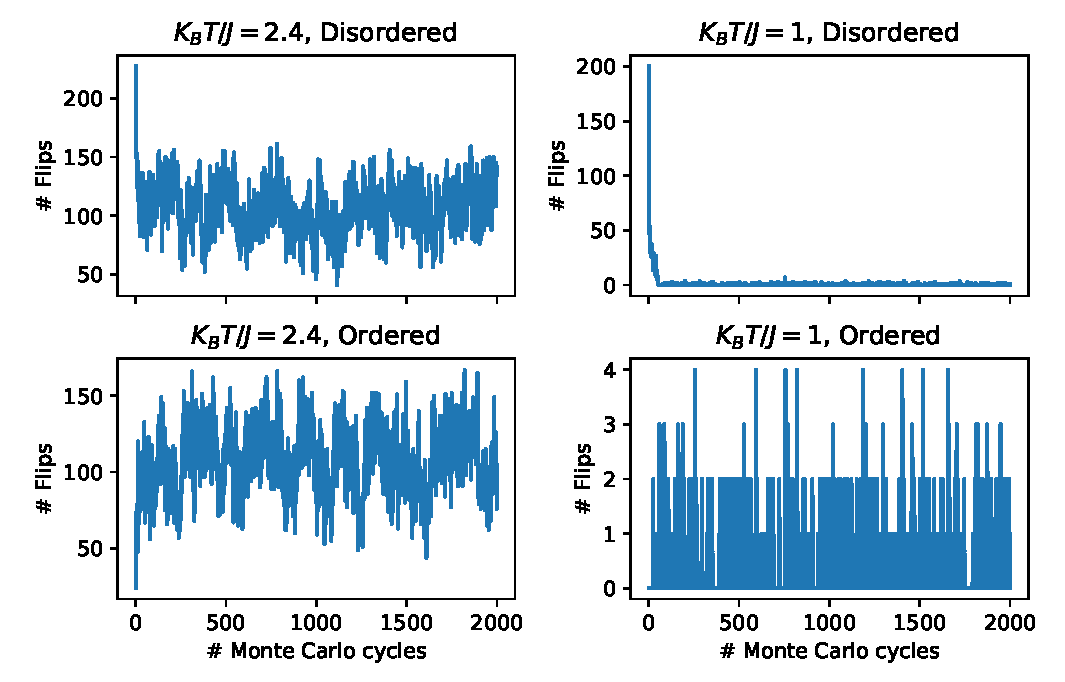
\includegraphics{{Figures/flip_MC1e7}.pdf}
	\caption{Figure showing the number of flips done to the spin values as a function of Monte Carlo cycles for a lattice with dimensions $N=20$. The simulations were done with two different temperatures $K_B T /J=1$ and $K_B T/J=2.4$ for and ordered lattice where all initial spins point in the same direction and an unordered lattice where all initial spins are chosen randomly.}
	\label{fig:flip_MC7}
\end{figure*}
The probability $P(E)$ was plotted for the two temperatures. This is shown in
Figure \ref{fig:histogram}. Here we started counting after $5000$ Monte Carlo
cycles to allow the solution to stabilize first. The variance $\sigma_E$ and variance
according to the central limit theorem $\sigma^2$ for this result is shown in
table \ref{tab:variances}.\\\\\indent
\begin{figure*}
	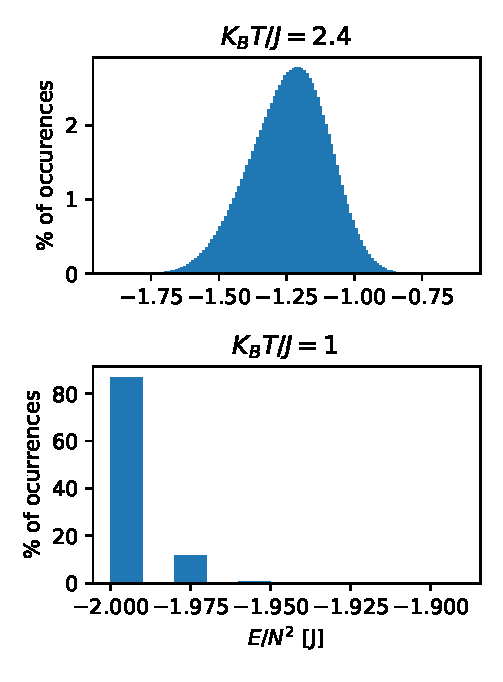
\includegraphics{{Figures/histogram}.pdf}
	\caption{Figure showing the probability $P(E)$ for a system with lattice size $N=20$ for two different temperatures $K_B T /J = 1.0$ and $K_B T/J = 2.4$. The energies were counted continously after $5000$ Monte Carlo cycles to allow the solution to stabilize.}
	\label{fig:histogram}
\end{figure*}
To study the behaviour of Ising model close to the critical temperature, the
mean energy $\langle E(T) \rangle$, heat capacity $C_v(T)$, magnetic susceptibility
$\chi(T)$ and the mean of the absolute value of the magnetization $\langle \vert
M(T) \vert \rangle$ was calculated in the interval $T\in\lbrack2.0, 2.5\rbrack$.
These thermodynamical quantities were plotted per particle in the given
interval with a timestep of $\Delta T=0.01$. This is shown in Figure
\ref{fig:thermo_quants}. For this calculation $10^6$ Monte Carlo cycles were
used for each temperature in the interval. The calculations were done on four
different lattice dimensions $N=40$, $N=60$, $N=80$ and $N=100$ to study how
this affects the solution. \\
The same calculation was also timed using a varying amount of threads for
parallisation and compiler flags for a lattice with dimensions $N=10$. This is
tabulated in table \ref{tab:timing}.
\begin{figure*}
	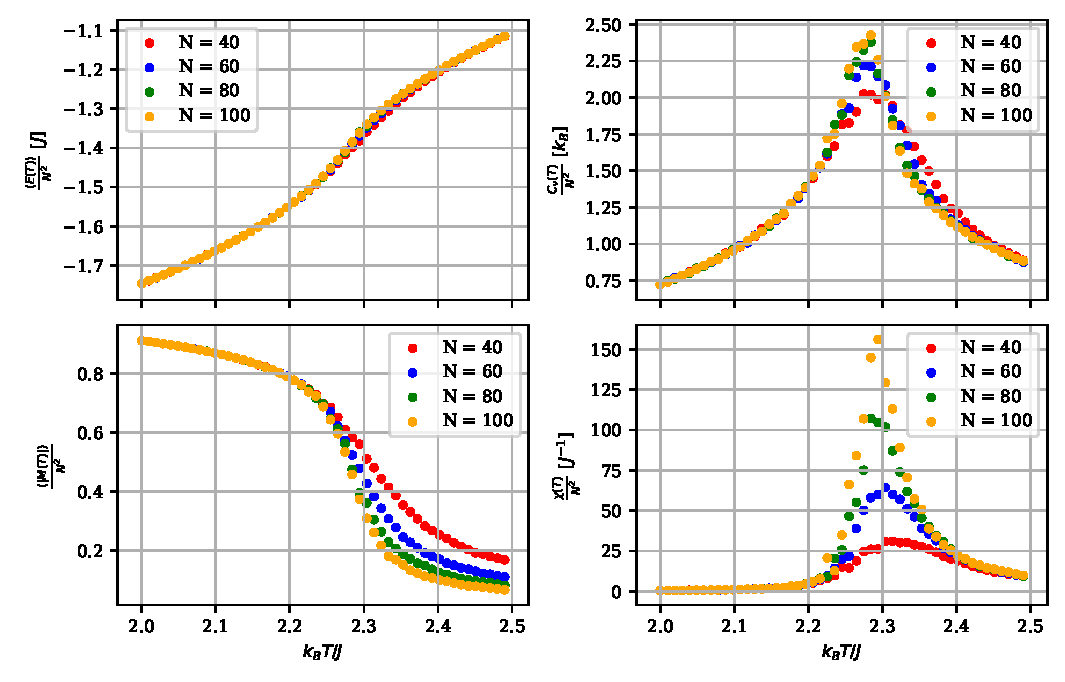
\includegraphics{{Figures/thermo_quants}.pdf}
	\caption{Figure showing thermodynamical quantitites per particle as a function of temperature for varying lattice dimensions $N$ after the solution has stabilized. Starting clockwise from the upper left the figure illustrates the mean energy $\langle E(T) \rangle$, heat capacity $C_v(T)$, magnetic susceptibility $\chi(T)$ and the mean of the absolute value of the magnetization $\langle \vert M(T) \vert \rangle$. The calculations were done with a temperature step $\Delta T = 0.01$.}
	\label{fig:thermo_quants}
\end{figure*}

\begin{deluxetable}{ccc}
	%\tablewidth{0pt}
	\tablecaption{Table showing the timing of a loop over 50 different temperatres using $10^6$ Monte Carlo Cycles for each loop iteration. The grid size for the lattice used was $N = 10$. \label{tab:timing}}
	%\tablecomments{}
	\tablecolumns{3}
	\tablehead{Threads & Flag & Run time [s]}
	\startdata
	1 & -O3 & 195.636 \\
	4 & -O3 & 55.539	\\
	8 & -O3 & 45.61	\\
	8 & -O1 & 220.689   
	\enddata
\end{deluxetable}

\begin{deluxetable}{lcc}
	%\tablewidth{0pt}
	\tablecaption{Table showing the variance in the energy $\sigma_E^2$ and the variance according to the central limit theorem $\sigma^2$ for to temperatures. The grid size used was $N = 20$ and $10^6$ Monte Carlo cycles with a sample start at 5000 cycles.\label{tab:variances}}
	%\tablecomments{}
	\tablecolumns{3}
	\tablehead{$k_BT / J$ & $\sigma_E^2$ $[J^2]$ & $\sigma^2$ $[J^2]$}
	\startdata
	1.0 & $5.848\cdot 10^{-5}$ & $5.848\cdot 10^{-12}$ \\
	1.4 & $0.0203$ & $2.03\cdot 10^{-9}$	
	\enddata
\end{deluxetable}
Finally we used the peaks of the heat capacity $C_v$ of the $N = 80$ and $N =
100$ lattices seen in Figure \ref{fig:thermo_quants}, to estimate the critical
temperature $T_C(N\to\infty)$ of an infinite grid according to the method
described in section \ref{subsec:analysis}. We found that the critical
temperature $k_BT_C / J \approx 2.284$ with a relative error to the
analytical value (by \cite{onsager:1944}) of $\epsilon \approx 0.675\%$.

\section{Discussion} \label{sec:discussion}

\section{Conclusion} \label{sec:conclusion}


\bibliography{ref}
\bibliographystyle{aasjournal}
\end{document}

% End of file `sample62.tex'.
